\section{引言}
工欲善其事,必先利其器。优秀的工具辅助,通常能使工作效率大幅度提升。
而我们今天所要介绍的Tbrowser Remote DevTools(Tbrowser远程页面调试工具)就是这样的利器。
它能使TV上页面调试工作拥有和PC上几乎一样的体验。
话不多说,让我们尽快开始Tbrowser Remote DevTools学习之旅吧。

\section{打开Tbrowser Remote DevTools}
为了保证浏览器性能,Tbrowser Remote DevTools是默认关闭的。
不过,只需要简单的操作就可以打开此功能。
我们提供两种方法打开Tbrowser调试功能:

\begin{itemize}
  \item \textbf{通过tcli命令打开}\\
  需要执行的命令是:/tvos/bin/tcli tbrw2.enabledevtools.pid\\
  pid是浏览器的进程号,可以通过 /tvos/bin/tcli help | grep tbrw2 命令查看。\\
  这种打开方式不需要重启TV,直接可以使用。但重启之后失效,还需再次执行命令。
  \begin{figure}[H] 
  \centering 
  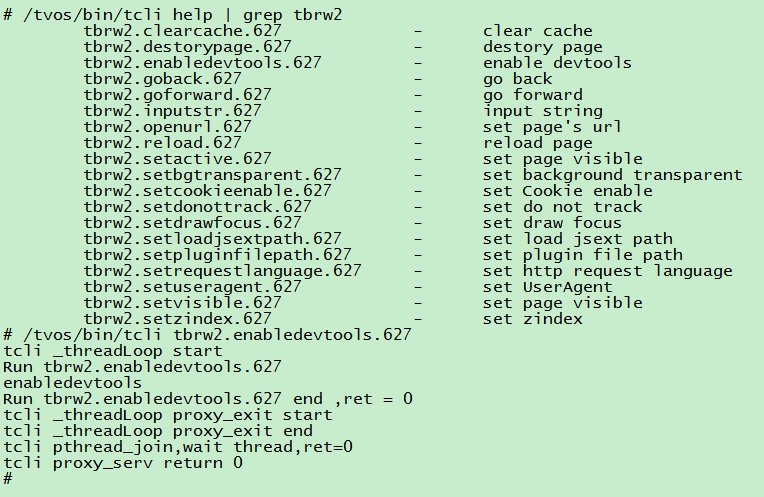
\includegraphics[width=0.9\textwidth]{image/devtools_study/tcli_command.PNG} 
  \caption{通过tcli打开过程} \label{fig:tcli_command} 
  \end{figure}
  
  \item \textbf{通过添加启动参数}\\
  需要添加的参数是:--remote-debugging-port=9222\\
  修改启动Tbrowser的run\_weblauncher\_server.sh脚本,添加上述的启动参数,重启TV即可。
  此种打开方式会一直打开Tbrowser Remote DevTools,重启依然有效,所以请不要在SQA的机器上这样修改。
\end{itemize}

Tbrowser Remote DevTools功能打开后,Tbrowser会监听指定的端口,创建一个http服务,供PC端访问。
可以通过 netstat -anp 命令查看系统的端口使用情况。
如果Tbrowser Remote DevTools功能开启,你将看到图\ref{fig:netstat_command}中的信息。
其中显示的IP是你机器的IP地址。如果使用tcli打开,端口默认是9222;如果添加了启动参数,那么端口就是参数中指定的端口号。
\begin{figure}[H] 
\centering 
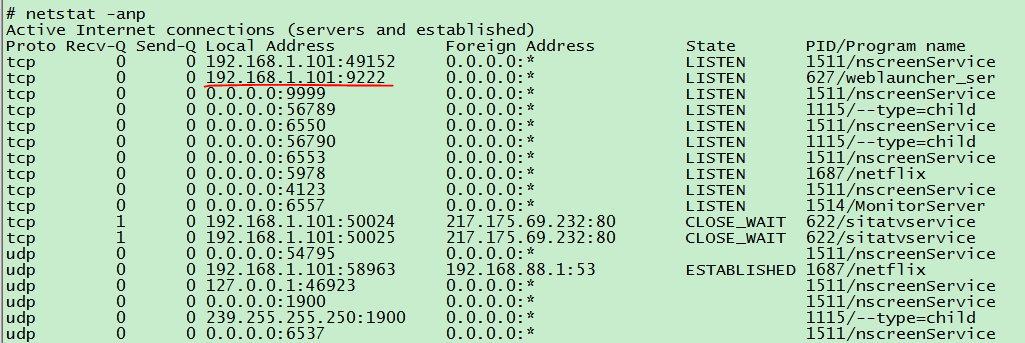
\includegraphics[width=0.9\textwidth]{image/devtools_study/netstat.PNG} 
\caption{netstat -anp命令输出结果} \label{fig:netstat_command} 
\end{figure}

到这里就非常接近成功了,后续要做的事情就是将PC连接到TV所在的网络(必须是直接连接,使用代理是不行的)。
打开PC上的Chrome浏览器,输出Tbrowser监听的地址,如上图应该是http://192.168.1.101:9222 。
如果一切顺利,你将看到图\ref{fig:home_page}中显示的内容。
其中BBC iPlayer、index.html、livetv、systemUi为打开的链接title。
如果此时浏览器没有打开任何页面,将没有任何链接。
\begin{figure}[H] 
\centering 
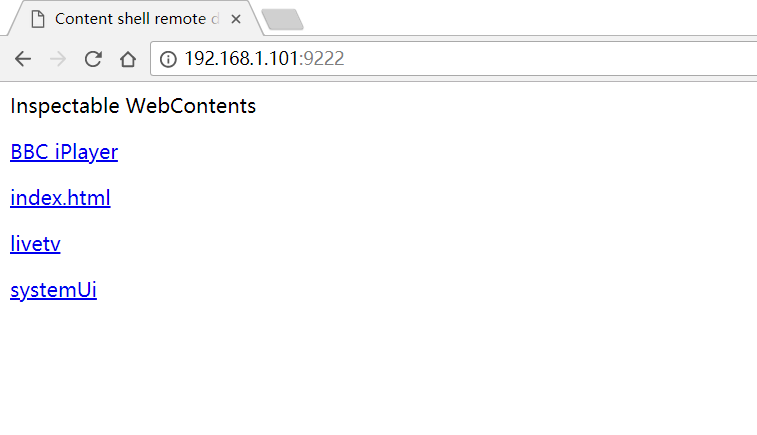
\includegraphics[width=0.9\textwidth]{image/devtools_study/home.PNG} 
\caption{Tbrowser Remote DevTools首页} \label{fig:home_page} 
\end{figure}

你可以点击其中的一个链接,进入调试页面,例如我打开BBC iPlayer链接,显示的效果如图\ref{fig:debug_page}所示。
至此,Tbrowser Remote DevTools功能已经准备妥当,下一步就可以进行页面调试了。
\begin{figure}[H] 
\centering 
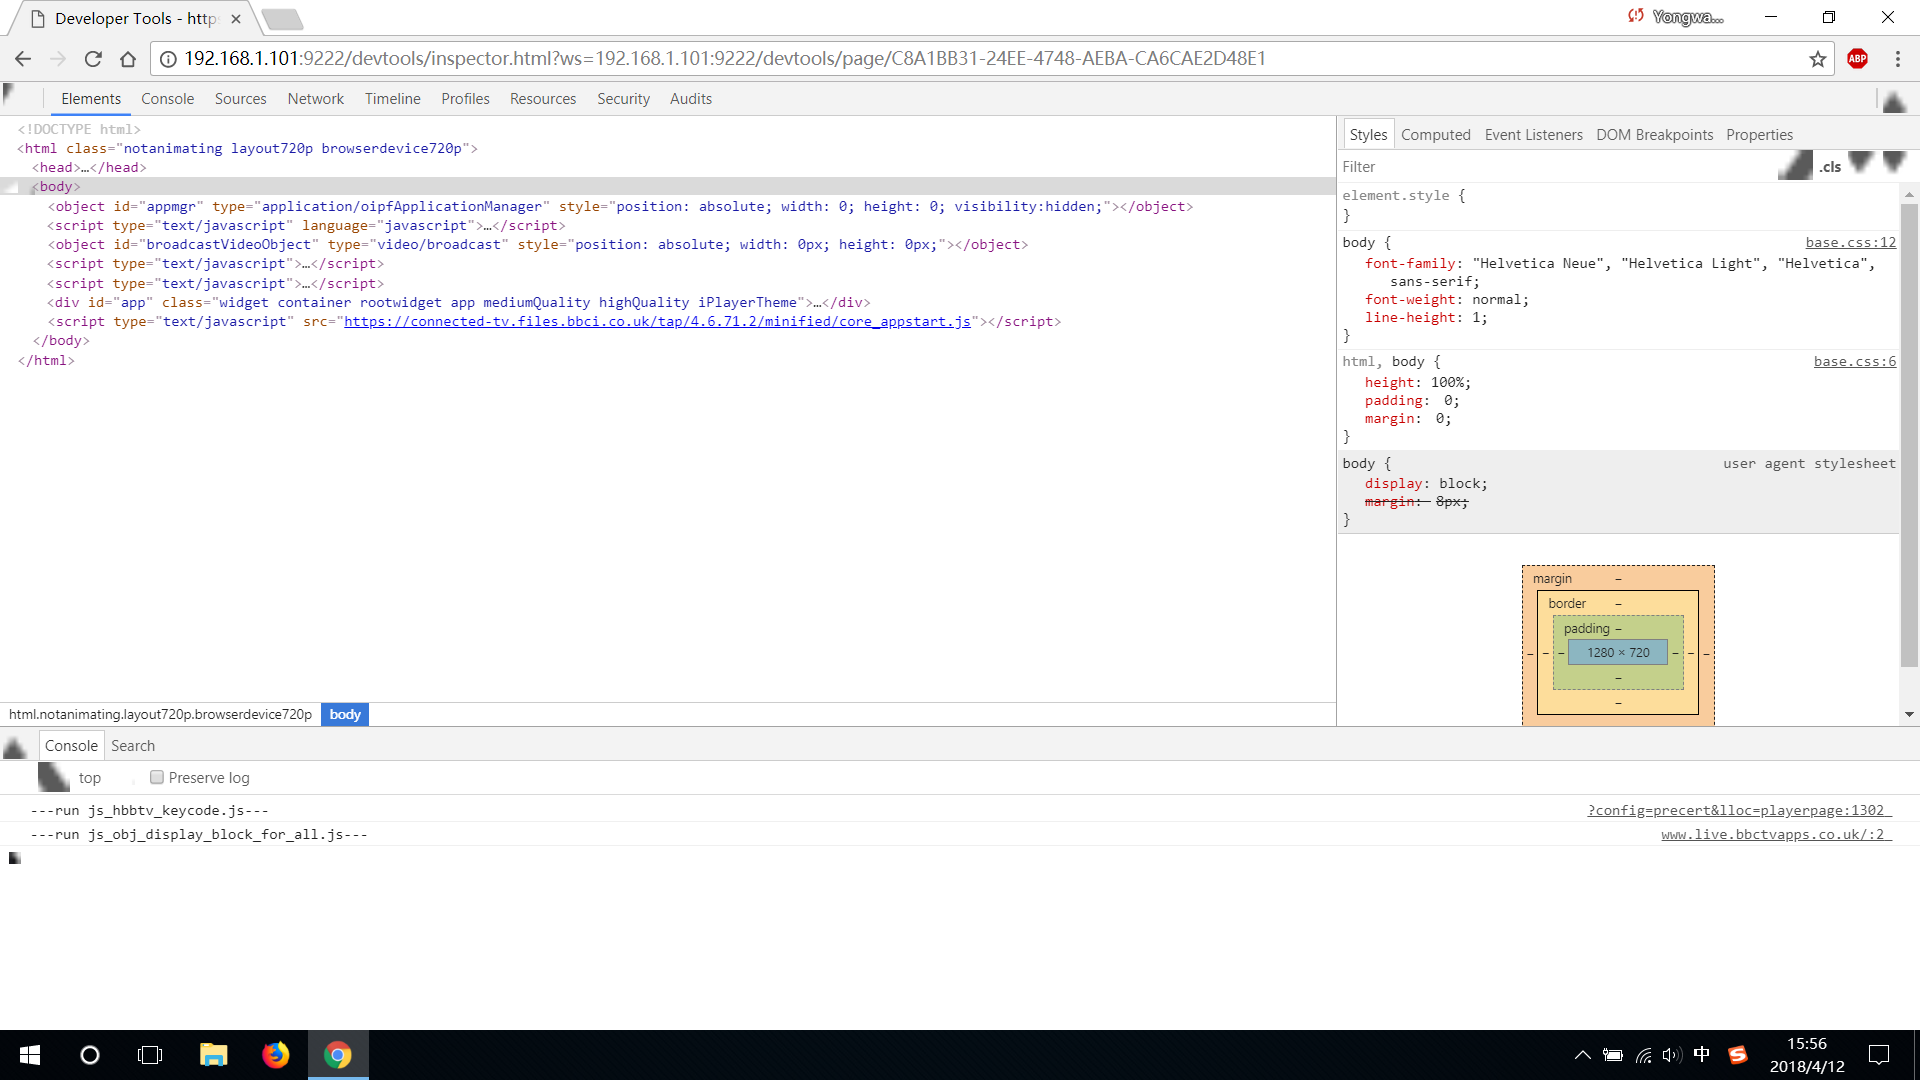
\includegraphics[width=0.9\textwidth]{image/devtools_study/debug_page.png} 
\caption{Tbrowser Remote DevTools调试页面} \label{fig:debug_page} 
\end{figure}

\section{使用Tbrowser Remote DevTools}
目前的Tbrowser2.0是基于Chromium49开发的,所以这里看到的调试页面是Chromium49版的调试页面。
有些功能和PC上的开发者工具不同,但大多数常用的功能还是一致的。
这里我们按照模块来研究一下Tbrowser Remote DevTools的具体使用情况。

\subsection{Elements面板}
Elements面板功能和最新的Chrome DevTools几乎没有区别,对于页面开发者来说这个模块的功能也应该非常熟悉。
Elements主要用于检查和实时编辑页面的 HTML 与 CSS。

\begin{figure}[H] 
\centering 
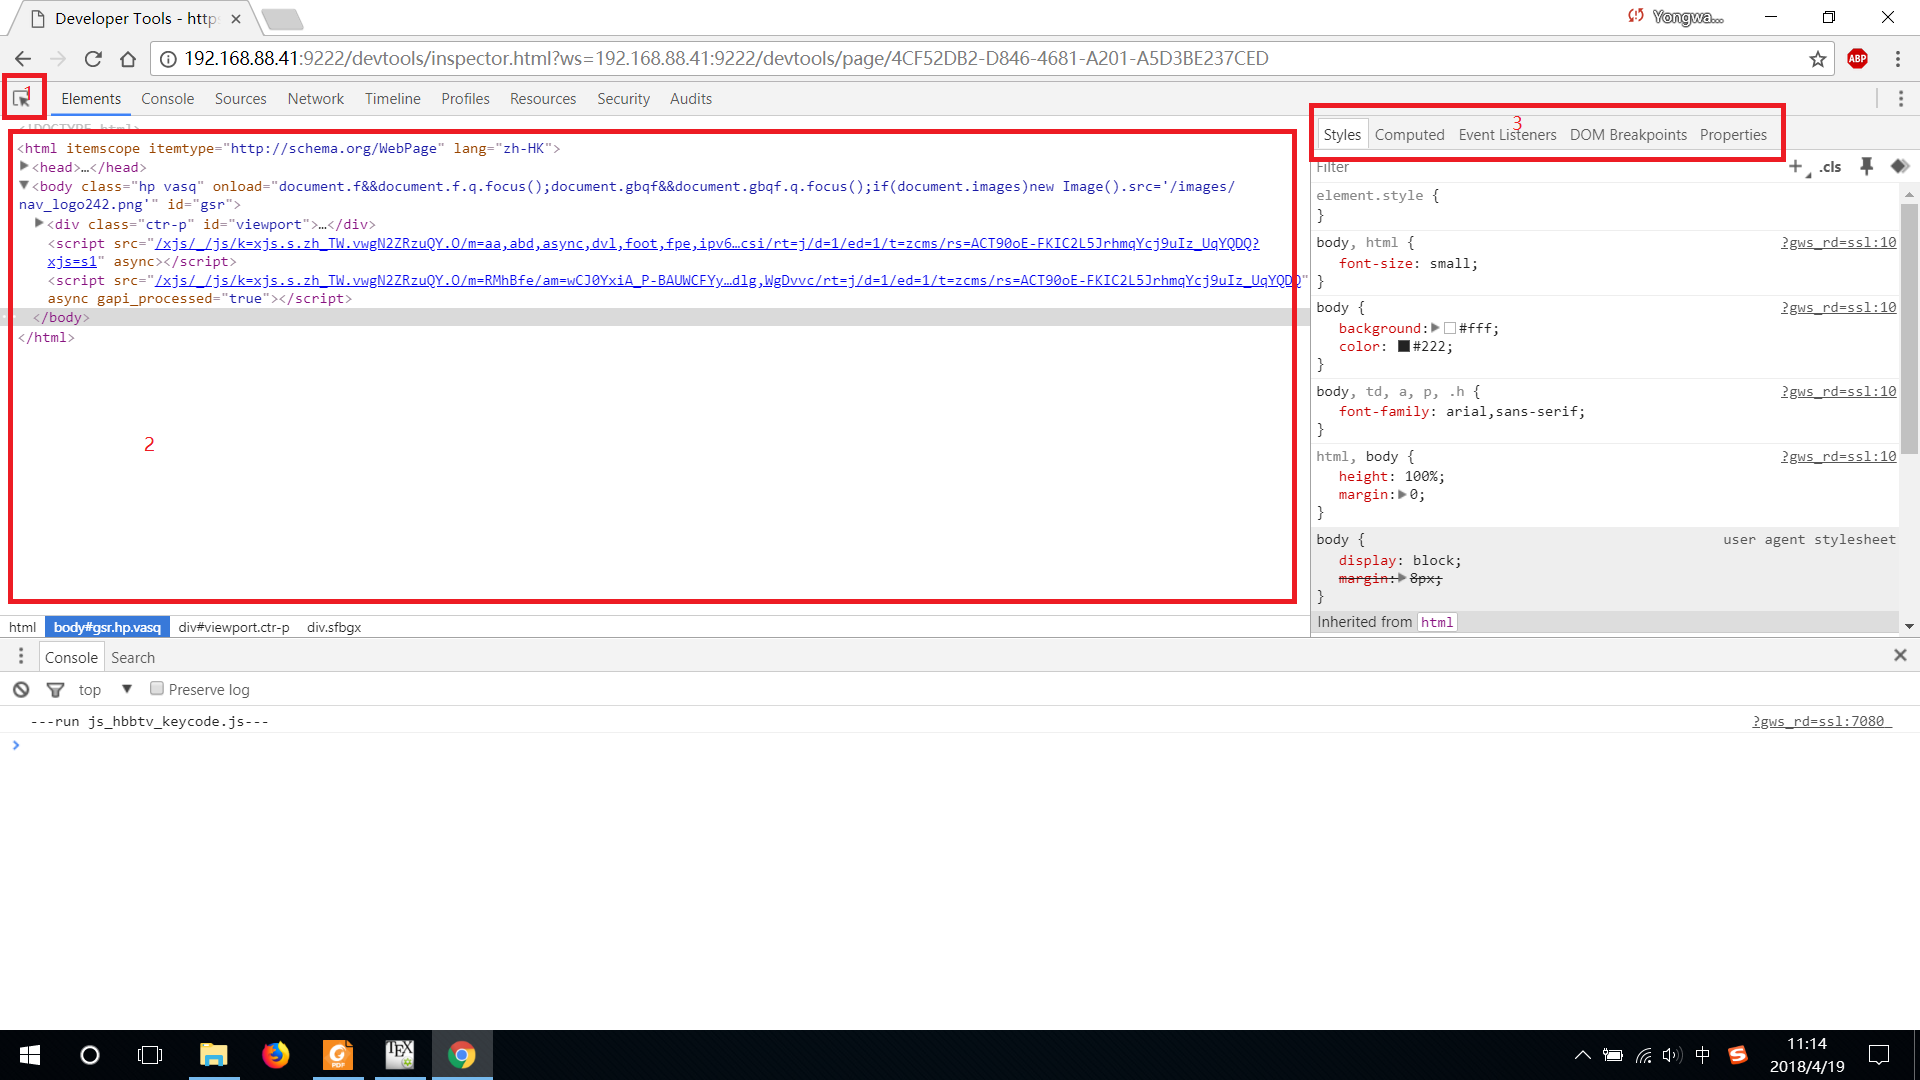
\includegraphics[width=0.9\textwidth]{image/devtools_study/elements_panel.png} 
\caption{DevTools Elements Panel} \label{fig:elements_panel} 
\end{figure}

如图\ref{fig:elements_panel}所示,是Elements面板的界面。
其中常用到的功能区已经在图中用红框标记出来了。
中间最大的红框2标记的区域是用来展示DOM树视图,这里的DOM树视图是经过JS执行之后的结果。
当鼠标移动到代码中的某个element上时,在TV上会使用不同的背景色高亮这些元素,并显示该元素的大小与位置坐标。

\begin{figure}[H] 
\centering 
\begin{minipage}[t]{0.45\textwidth}
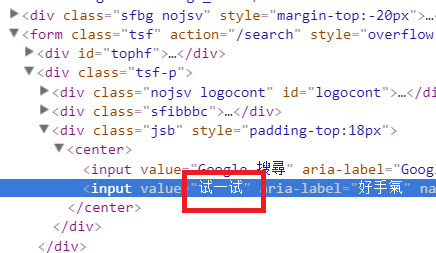
\includegraphics[width=0.9\textwidth]{image/devtools_study/elements_edit_code.png} 
\caption{修改Google页面代码}
\end{minipage}
\begin{minipage}[t]{0.45\textwidth}

\includegraphics[width=0.9\textwidth]{image/devtools_study/elements_edit_result.png} 
\caption{修改Google页面效果}
\end{minipage}
\end{figure}

双击HTML代码可以进行编辑文本,或者右键选择Edit as HTML(快捷键是F2)进行编辑,编辑后的页面会同步更新。
如图\ref{fig:modify_google}就是将google页面中的“好手气”改为“试一试”之后的效果。

\begin{figure}[H] 
\centering 
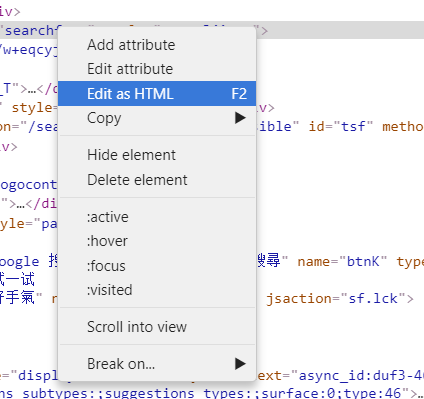
\includegraphics{image/devtools_study/element_right_menu.png} 
\caption{Elements右键菜单} \label{fig:element_right_menu} 
\end{figure}

另外,如图\ref{fig:element_right_menu}在这个区域的右键菜单中还提供了一些其他功能,下面也做出一些简要说明:
\begin{itemize}
\item Add attribute: 为选中的元素添加一个属性。
\item Edit attribute: 编辑鼠标所在位置的属性,与双击鼠标作用相同。
\item Edit as HTML: 编辑HTML代码,会打开一个编辑框进行代码编辑。点击编辑框以外的部分或者Esc键可以退出编辑模式。
\item Copy: 在远程调试中Copy是不可用的。在调试过程中,可以复制文本,但不能使用任何的Copy或Save功能。
因为这些命令会发送到TV端执行,而Server端禁止执行这些命令。
\item Hide element: 隐藏或取消隐藏选中的元素。
\item Delete element: 删除选中的元素。注意:在远程调试中element一旦删除,无法撤销,只有重新加载页面才能恢复。
\item :active :hover :focus :visited : 强制修改页面伪状态。
\item Scroll into view:控制选中的element对应的页面元素滚动到可见区域。
\item Break on ...: 添加Dom Breakpront。关于Dom Breakpront会在讲解Sources模块时详细说明。
\end{itemize}

图\ref{fig:elements_panel}中左上角的红框1标记出图标的功能是通过点击页面元素,来定位其在代码中的位置。
这个功能和Chrome的Devtools的功能一样。只不过有一个前提就是打开这个页面的应用要响应鼠标事件。
此功能的快捷键是Ctrl+Shift+C。

图\ref{fig:elements_panel}中右上角的红框3标记出来的一系列Tabs是用来查看代码区选中element的各项属性的。
下面简要介绍一下各个标签的作用:
\begin{itemize}
\item Styles 用于展示对选中的element的CSS属性。其中包含对其自身或者其父节点的CSS属性设置。
没有生效的属性会使用横线划掉表示。
在这个标签内可以勾选每条属性前的复选框来改变页面中的节点CSS属性,也可以直接编辑。
\item Computed 用于展示选中element计算之后的CSS属性,这里会列出该element所有被设置的属性。
展开其中的一条属性可以看到在这个节点上对该属性所有设置的值和设置的代码位置。
没有生效的值会使用横线划掉。Computed 标签内的值不能修改。
\item Event Lisenters 用于展示选中的element监听的JS事件。
展开其中一条事件可以看到事件监听方法在代码中的位置,点击代码路径可以调整到对应的函数。
这个标签用于调试JS事件的处理情况非常方便。
\item Dom Breakpronts 用于展示和管理Dom Breakpront。关于Dom Breakpront会在讲解Sources模块时详细说明。
\item Properties 用于展示选中的element所有的property。其中包含了element自身和它的原型链的所有property。
\end{itemize}

更多信息可以查看Chrome Devtools说明文档:https://developers.google.com/web/tools/chrome-devtools/inspect-styles/?hl=zh-cn

\subsection{Console面板}
Chrome DevTools的Console面板主要有两个功能:查看页面log信息和执行命令。
但是目前Tbrowser Remote DevTools只支持查看页面log的功能,暂时不支持命令的执行。

\begin{figure}[H] 
\centering 
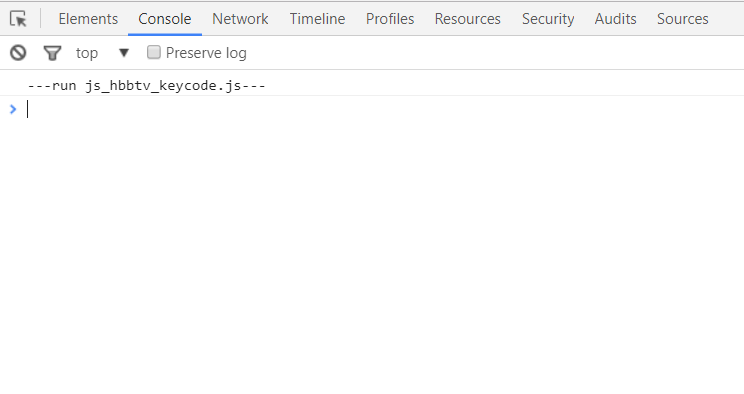
\includegraphics[width=0.9\textwidth]{image/devtools_study/console_panel.png} 
\caption{Console界面} \label{fig:consloe_panel} 
\end{figure}

如图\ref{fig:consloe_panel}所示,是Console的界面。
其中上面的一排按钮的功能分别为:
\begin{itemize}
\item Clear conlose 清除log,用于清除当前Console界面中的log。快捷键是Ctrl+L。
\item Filter 用于根据输入的关键字过滤log信息,支持正则表达式。
\item iframe 选择iframe,如果页面使用多个iframe,可以通过这里切换iframe。top是main frame;默认为当前操作的iframe。
\item Preserve log 保持log,如果勾选此选项,那么在页面切换或者重新加载是不会清除以前的log信息。
\end{itemize}

\begin{figure}[H] 
\centering 
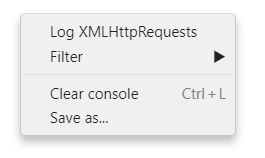
\includegraphics{image/devtools_study/consloe_right_menu.png} 
\caption{Console界面} \label{fig:consloe_right_menu} 
\end{figure}

如图\ref{fig:consloe_right_menu}所示,在Console的右键菜单中还提供了一些功能:
\begin{itemize}
\item log XMLHttpRequest 如果勾选此选项会在执行XMLHttpRequest时输出log。
\item Fileter 此功能和按钮的功能不一样,这里是用于隐藏某个文件中所有的log。
\item Clear conlose 和按钮的功能一致。
\item Save as... 此功能不可用。
\end{itemize}

更多信息可以查看Chrome Devtools说明文档:https://developers.google.com/web/tools/chrome-devtools/console/?hl=zh-cn

\subsection{Sources面板}
Sources面板主要用于页面代码的浏览器与调试,主要是对JavaScript代码的调试使用较多。

\begin{figure}[H] 
\centering 
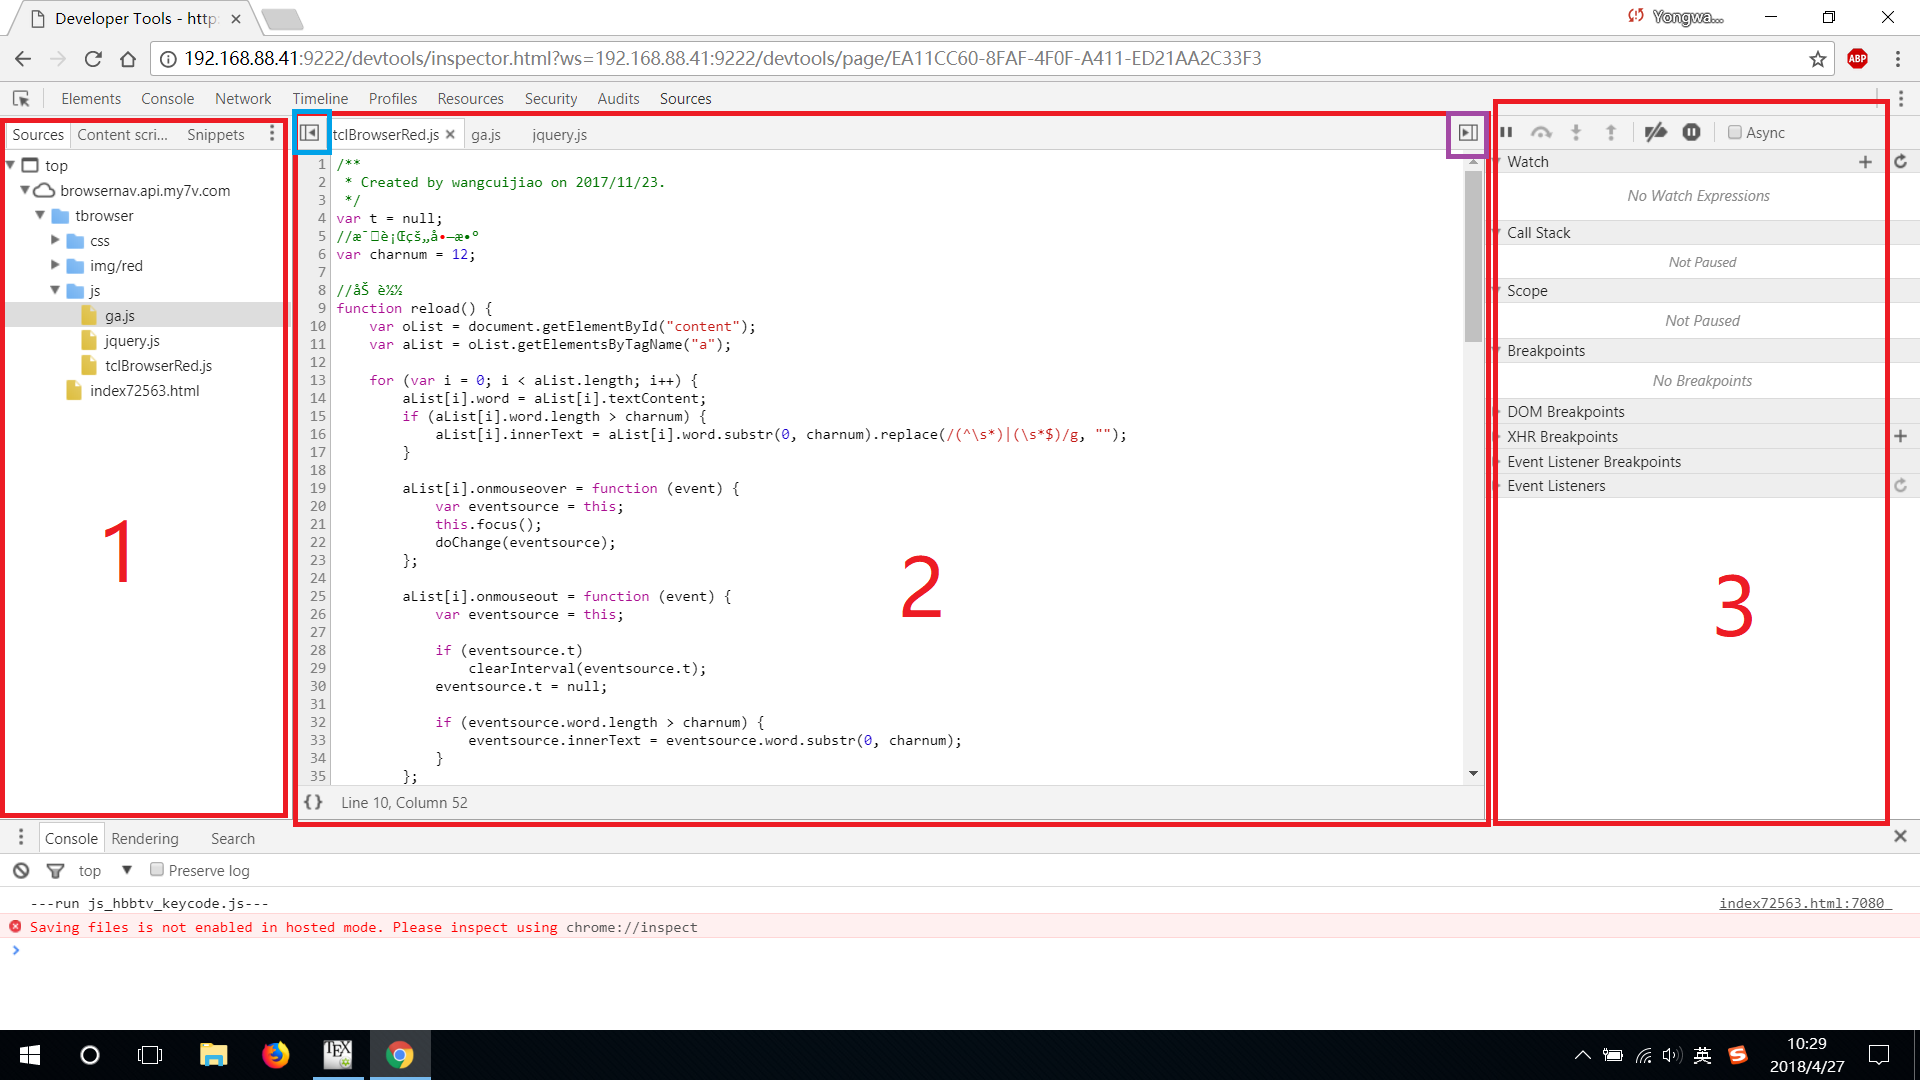
\includegraphics[width=0.9\textwidth]{image/devtools_study/sources_panel.png} 
\caption{Sources界面} \label{fig:sources_panel} 
\end{figure}

如图\ref{fig:sources_panel}所示,是Sources界面。
如图中的红框标记,Sources界面主要分为三个区域。
\begin{itemize}
\item 红框1标记出的左侧工具栏用于文件浏览,默认是按照文件夹的结构显示的。
\item 红框2标记出的中间区域用于代码浏览和调试。
其中左上角和右上角的两个按钮用于显示和隐藏左右工具栏。
左下角的大括号图标用于格式化JS代码。
\item 红框3标记胡的右侧工具栏用于查看调试过程中的变量、堆栈和管理断点。
\end{itemize}

在开始熟悉JavaScript调试之前,了解一下JavaScript调试的入门知识非常有好处。
Chrome Devtools说明文档中《在 Chrome DevTools 中调试 JavaScript 入门》就是一个不错的教程,链接是:https://developers.google.com/web/tools/chrome-devtools/javascript/?hl=zh-cn。为了方便我将其内容添加到这里。

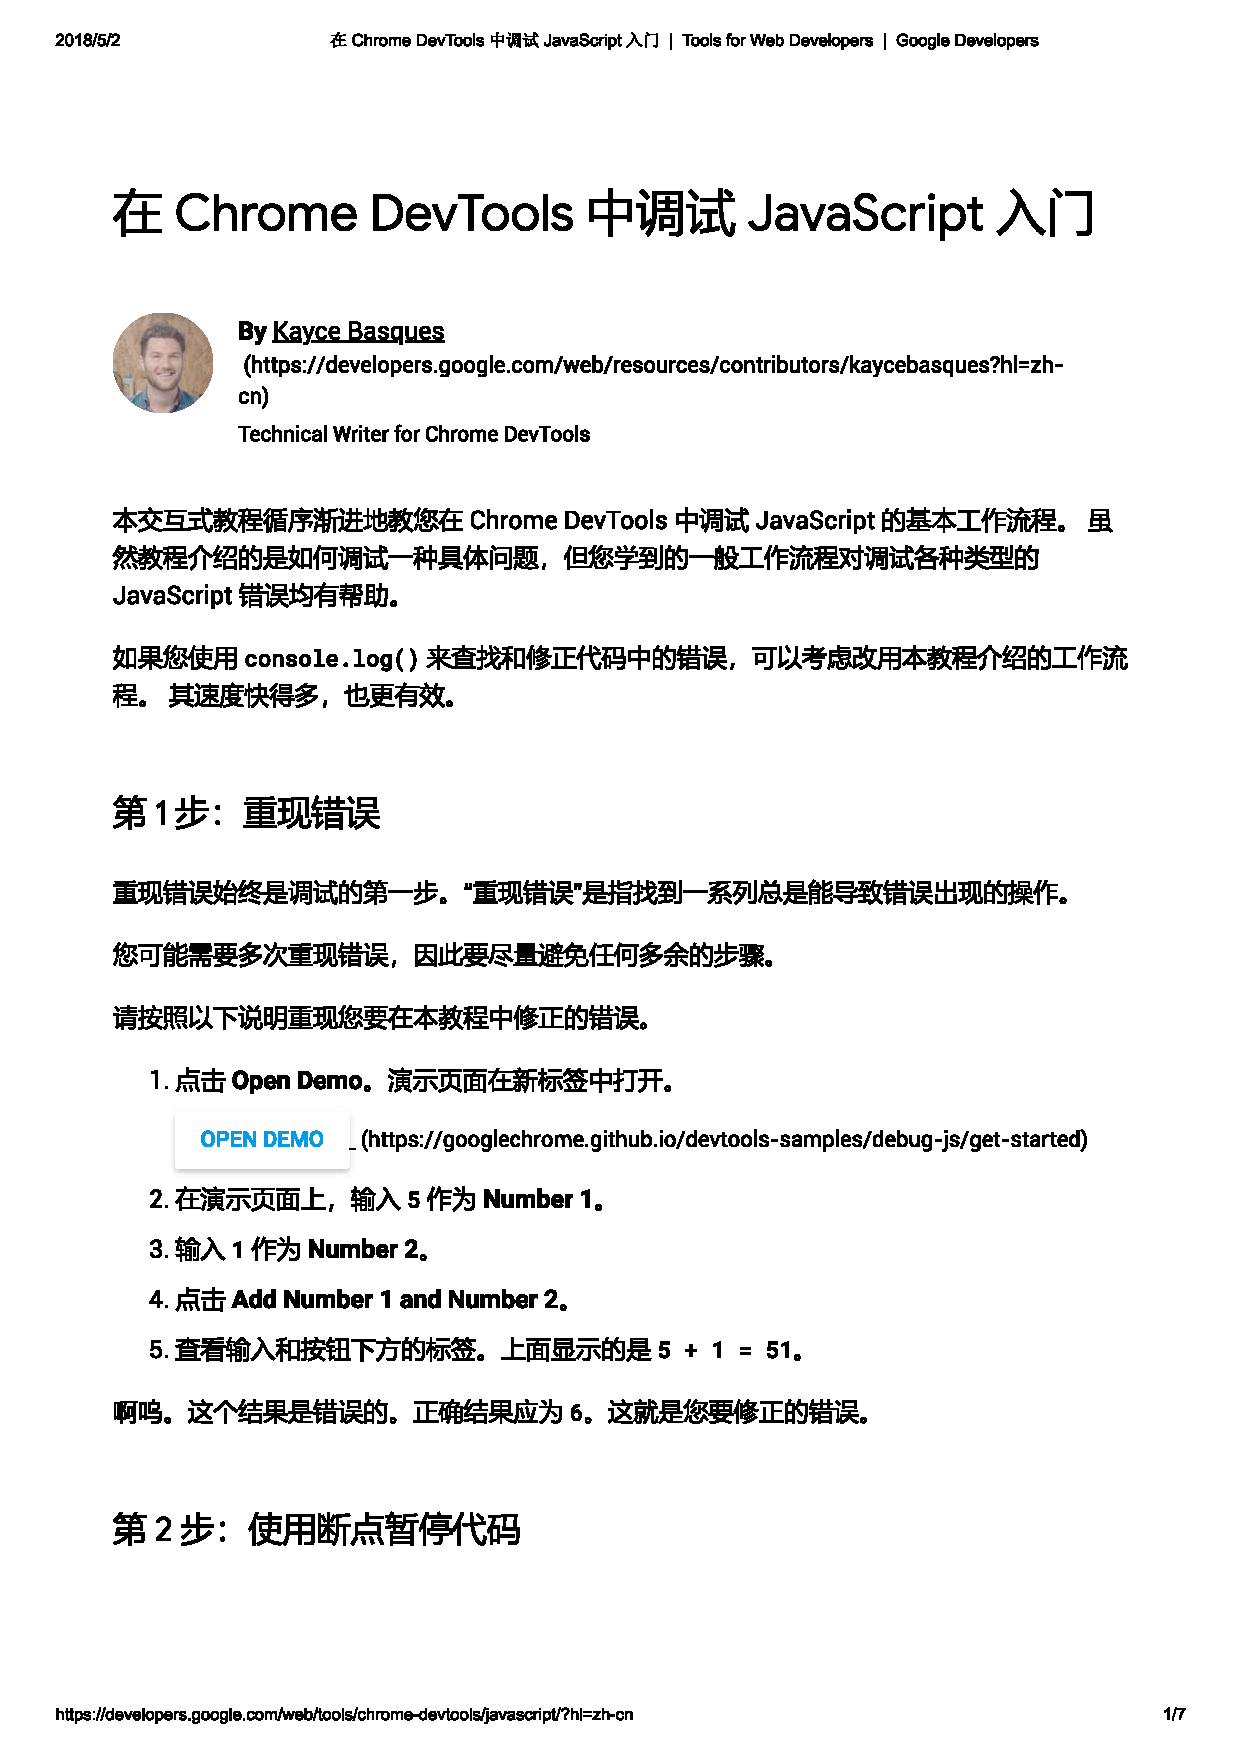
\includepdf[pages={1,2,3,4,5,6}]{image/devtools_study/javascript_debug.pdf} 

下面的内容,我们重点了解一下如何添加断点。
在Tbrowser Remote Devtools中支持以下七种断点:

\begin{tabular}{|l|p{10cm}|}
\hline
Line-of-code & 在代码中的确切位置添加断点\\
\hline
Conditional line-of-code & 在代码中的确切位置添加条件断点,只有条件表达式运算结果为true才会生效\\
\hline
DOM & 当更改或者移除特定的DOM节点或者其子节点时触发的断点 \\
\hline
XHR & 当一个XHR请求的URL包含指定的字符串时触发的断点 \\
\hline
Event listener & 当一个事件(如keydown、click)发生时触发的断点 \\
\hline
Exception & 当捕获到异常信息时发出的断点 \\
\hline
Function & 当特定函数执行时触发的断点 \\
\hline
\end{tabular}

\subsubsection{Line-of-code Breakpoints}
确切断点一般用于知道要调试代码的确切位置时使用。
在代码中的某一行添加断点后,当执行到这一行之前JavaScript代码的执行就会被暂停。

添加确切断点的方法有两种:
\begin{itemize}
\item 在JavaScript代码的左侧行号位置鼠标左键单击。行号背景色会变为蓝色,断点就添加成功了。
\item 在代码中调用debugger。调用debugger后,正常打开页面不会暂停代码执行。
需要在Devtool打开的情况下,执行到debugger语句时就会暂停执行不需手动添加断点。
\end{itemize}

\begin{figure}[H] 
\centering 
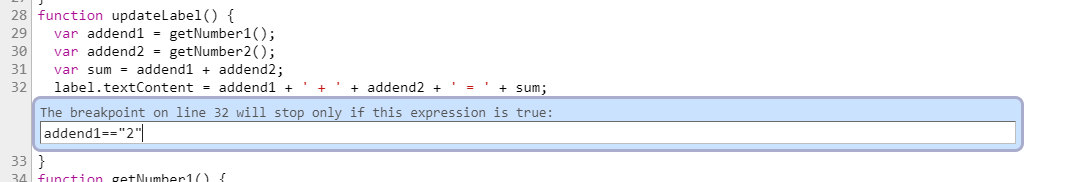
\includegraphics[width=0.9\textwidth]{image/devtools_study/add_conditional_breakpoint1.png} 
\caption{添加条件断点} \label{fig:sources_panel} 
\end{figure}

\begin{figure}[H] 
\centering 
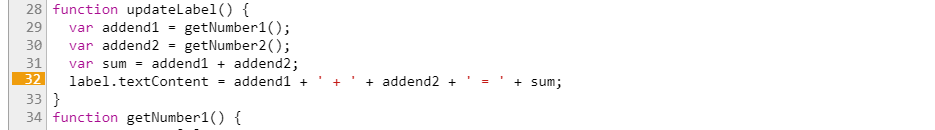
\includegraphics[width=0.9\textwidth]{image/devtools_study/add_conditional_breakpoint2.png} 
\caption{添加添加断点成功} \label{fig:sources_panel} 
\end{figure}

如果想要只在某种条件下才出发断点,可以使用条件断点。添加条件断点的步骤是:
\begin{enumerate}
\item 在要添加条件断点的行号处右键,选择Add conditional breakpoint...。
\item 在条件编辑框内输入触发的条件。输入Tab键或者鼠标点击其他区域完成编辑。
\item 此时对应行号的背景色会变为橙色,表明条件断点已经添加成功。
\item 在条件断点处右键可以编辑条件和删除断点。
\end{enumerate}

在右侧工具栏中的Breakpoints标签中可以查看和管理所有的确定断点。
其中常用的操作有:
\begin{itemize}
\item 停用/启动断点。勾选断点前的复选框可以停用/启用单个断点;右键菜单中可以停用/启用所有断点。
\item 删除断点。右键菜单中可以删除单个或者全部断点;单击已经添加的断点的行号也可以删除断点。
\item 定位断点所在位置。单击单个断点可跳转断点在代码中的位置。
\end{itemize}

\subsubsection{DOM Breakpoints}
Dom断点是当页面指定的节点或者其子节点被删除或更改时触发的断点。
代码将暂停在修改指定节点的JavaScript代码中。
添加Dom断点的步骤是:
\begin{enumerate}
\item 打开Elements面板,选择要检测的元素。
\item 在右键菜单中选择Break on...。
\item 再在子菜单中选择添加断点的类型。
\item 添加成功后会在Dom树的左侧有一个蓝色的小点标记。
\end{enumerate}

\begin{figure}[H] 
\centering 
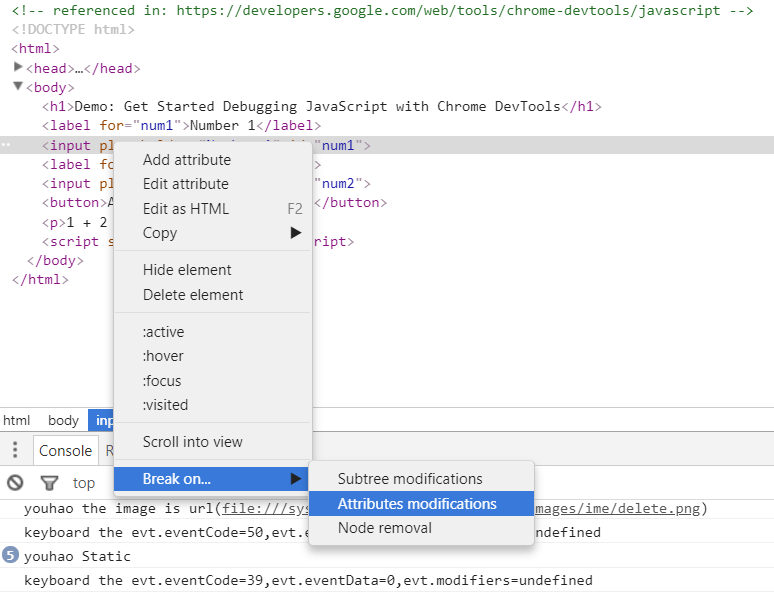
\includegraphics[width=0.9\textwidth]{image/devtools_study/add_dom_breakpoint.png} 
\caption{添加Dom断点的过程} \label{fig:sources_panel} 
\end{figure}

Devtools支持三种Dom断点:
\begin{itemize}
\item Subtree modifications: 当选中的节点的子节点被删除或添加,或者子节点的内容发生改变时触发断点。
当子节点的属性或选中节点的属性和内容发生变化时不会触发断点。
\item Attributes modifications: 当选中节点的属性被添加、删除或者属性值发生变化时触发断点。
\item Node Removal: 当选中的节点被删除时触发断点。
\end{itemize}

\subsubsection{XHR Breakpoints}

\subsection{Network模块}
\subsection{Timeline模块}
\subsection{Profiles模块}
\subsection{Resourcess模块}
\subsection{Security模块}
\subsection{Audits模块}